
\documentclass[a4paper]{article}
\usepackage{interlude}
\usepackage{pslatex}
\usepackage[T1]{fontenc}
\usepackage[utf8]{inputenc}
\usepackage{verbatim}
\usepackage{amssymb}
\usepackage{tikz}
\usepackage{multicol}

\newenvironment{inscore}	{\vspace{-2mm}\small\verbatim}{\endverbatim\vspace{-2mm}}
\newcommand{\OSC}[1]		{\texttt{#1}}

\tikzstyle{box}=[rectangle,draw,fill=white!50,text=black] 
\tikzstyle{child}=[->,very thick,>=latex]
\tikzstyle{refers}=[->,dotted,very thick,>=latex]

\makeatother

\begin{document}

\title{Graphic rendering of audio processing specification \\ v.1.06}

\author{Grame \\ Centre national de cr\'eation musicale}

\maketitle

%=============================================== INTRO ===================================================
\section*{Introduction}\label{sec:intro}

The aim of this specification is to define the possible representations of musical processes through INScore objects. For now, it is already possible for the score components to evolve following time messages, such as a clock or a piece of music, but this remains only possible for the synchronized objects, and they are simply moved (sometimes stretched) to fit their master's mapping. All other informations than time are not represented. We now would like to imagine an object changing size, orientation, color, transparency, etc. following the values of a signal. Therefore, we will first expose the existing tools to create signals in INScore and then see how we could use them to control any characteristic of any object following a signal.

\section{The signals in INScore}\label{sec:signals}

As said before, it is already possible to represent incoming signals in INScore, but they are only meant to be drawn as graphical signals and not to control arbitrary  components'properties.

For now, any object possesses a static node that can be seen as a container of all signals possibly present in the object. Those signals can be simple or more complex (parallel signals) and they are read by a graphical signal on the same level of hierarchy than our signal node.

\begin{figure}[h]
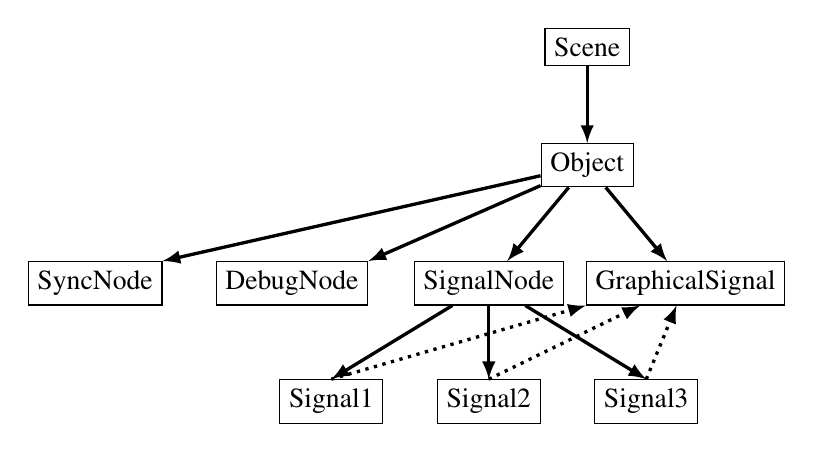
\begin{tikzpicture}

  \node[box] (S) at (1.25,3) {Scene};
  \node[box] (O) at (1.25,1.5) {Object};
  \node[box] (DN) at (-2.5,0) {DebugNode};
  \node[box] (SyN) at (-5,0) {SyncNode};
  \node[box] (SN) at (0,0) {SignalNode};
  \node[box] (GS) at (2.5,0) {GraphicalSignal};
  \node[box] (s1) at (-2,-1.5) {Signal1};
  \node[box] (s2) at (0,-1.5) {Signal2};
  \node[box] (s3) at (2,-1.5) {Signal3};
  
  \draw[child] (S)--(O);
  \draw[child] (O)--(DN.north east); \draw[child] (O)--(SyN.north east); \draw[child] (O)--(SN); \draw[child] (O)--(GS);
  \draw[child] (SN)--(s1.north); \draw[child] (SN)--(s2.north); \draw[child] (SN)--(s3.north);
  \draw[refers] (s1.north)--(GS.south west);  \draw[refers] (s2.north)--(GS);  \draw[refers] (s3.north)--(GS);
    
\end{tikzpicture}

 \caption{The Signal Node}
 \label{fig:signalNode}
\end{figure}


\section{Linking a signal to an object's property}\label{sec:link}

There could be several ways to define the connection between signals and attributes in INScore. First of all because a signal can have a dimension greater than 1 (composed of several simple signals) and the attributes as well (like a color - H, S, B, A or R, G, B, A - or  a position - x, y, z). 

We could imagine the largest and most permissible syntax possible : that would be linking a $n-dimensional$ signal to a $m-dimensional$ attribute, and handle the different cases for $n \neq{} m$. 

But, considering there are really few $m-dimensional$ attributes, and that each of those can be decomposed in "sub-attributes" (for instance R, G, B, and A for a color) that can me modified independently, we saw no reason why the notations should be more complex, when we could choose to simplify it at the most : One signal connected to one or more attribute(s) with a single dimension (Figure \ref{fig:linking}). The color and the position will then have to be linked for each "sub-attribute", and not as a whole.
\\

\begin{figure}[h]
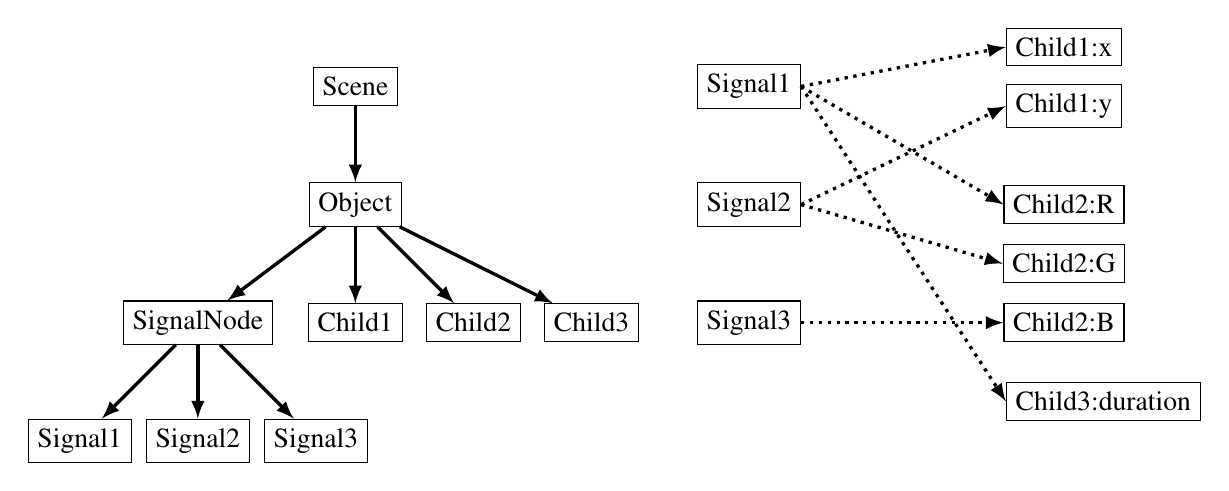
\begin{tikzpicture}

  \node[box] (S) at (2,3) {Scene};
  \node[box] (O) at (2,1.5) {Object};
  \node[box] (SN) at (0,0) {SignalNode};
  \node[box] (C1) at (2,0) {Child1};
  \node[box] (C2) at (3.5,0) {Child2};
  \node[box] (C3) at (5,0) {Child3};
  \node[box] (s1) at (-1.5,-1.5) {Signal1};
  \node[box] (s2) at (0,-1.5) {Signal2};
  \node[box] (s3) at (1.5,-1.5) {Signal3};
  
  \node[box] (S1) at (7,3) {Signal1};
  \node[box] (S2) at (7,1.5) {Signal2};
  \node[box] (S3) at (7,0) {Signal3};
  
  \node[box] (C1a1) at (11,3.5) {Child1:x};
  \node[box] (C1a2) at (11,2.75) {Child1:y};
  \node[box] (C2a1) at (11,1.5) {Child2:R};
  \node[box] (C2a2) at (11,0.75) {Child2:G};
  \node[box] (C2a3) at (11,0) {Child2:B};
  \node[box] (C3a1) at (11.5,-1) {Child3:duration};
  
  \draw[child] (S)--(O);
  \draw[child] (O)--(SN); 
  \draw[child] (SN)--(s1); \draw[child] (SN)--(s2); \draw[child] (SN)--(s3);
  \draw[child] (O)--(C1); \draw[child] (O)--(C2); \draw[child] (O)--(C3);
  
  \draw[refers] (S1.east)--(C1a1.west); \draw[refers] (S2.east)--(C1a2.west); 
  \draw[refers] (S1.east)--(C2a1.west); \draw[refers] (S2.east)--(C2a2.west); \draw[refers] (S3.east)--(C2a3.west);
  \draw[refers] (S1.east)to(C3a1.west);
      
\end{tikzpicture}

 \caption{Example of connections between signals and attributes}
 \label{fig:linking}
\end{figure}



The signal node will receive the connection messages and store all the links between signals and attributes in a map of the form :
\begin{center}
< \textit{std::string}  object:attribute[range], \textit{ParallelSignal} signal >
\end{center}


The syntax chosen for the OSC message is :

\begin{center}
\OSC{/ITL/scene/.../object/signal connect mySig myChild1:myAttribute1[r1,r2]:myAttribute2[r1',r2']:myAttribute3 myChild2:myAttribute1 }
\end{center}


Where r1 and r2 are optional range bounds to specify the range of our values if different from the default ones.
\\

Indeed, by default a signal will have a range of [-1, 1]. For some attributes, such as the position, the dimensions or the scale, those values stay exactly the same, because they correspond to our graphical space. Nonetheless, there are some attributes that must have another default range, the [-1,1] range having no meaning for them : the date, the duration, the angle, the color...
%
%The table \ref{ranges} gives us the default data range corresponding to the signal float range [-1, 1] .
%
%\begin{table}[htdp]
%\begin{center}
%\begin{tabular}{|r|c|c|}
%\hline
%Attribute & attribute's range\\
%\hline
%\OSC{x, y, z} [position] 	& [-1,1]\\
%\OSC{width, height} [dimension] 	& [-1,1] \\
%\OSC{scale} 		& [-1,1] \\
%\OSC{date} 		& [0,1]\\
%\OSC{duration} 	& [0,1] \\
%\OSC{angle}		& [0,360] \\
%\OSC{rotatex, rotatey, rotatez} 		& [0,360] \\
%\OSC{red, green, blue, alpha}			& [0,255] \\
%\OSC{hue}  		& [0,360]\\
%\OSC{saturation}  	& [0,100] \\
%\OSC{brightness}  	& [0,100] \\
%\hline
%\end{tabular}
%\end{center}
%\caption{Attributes ranges corresponding to the signal range [-1,1].}
%\label{ranges}
%\end{table}%

However, the bounds \OSC{r1} and \OSC{r2} will allow us to change the range to fit the incoming signals or the dimension of our attributes. For example, if a cursor is synchronized on a score, we could set the range of variation of our cursor's date to the score duration, so that the values of the signal can make it move on the whole score.

\section{Handling the attributes}\label{sec:handler}

As the OSC Message that each object receives are computed by message handlers (IMsgHandler), we are going to create a signal handler class (ISigHandler), in order to call the corresponding setting method for each object's attribute. 
Those handlers will be created at the object's construction, just like the others, and they will be called by a method IObject::executeSignal(\textit{std::string} method, \textit{ParallelSignal} signal). The figure \ref{fig:handler} shows us the way the OSC messages are handled, and how we should handle the signals.
\\

\begin{figure}[h]
\hspace{-3cm}
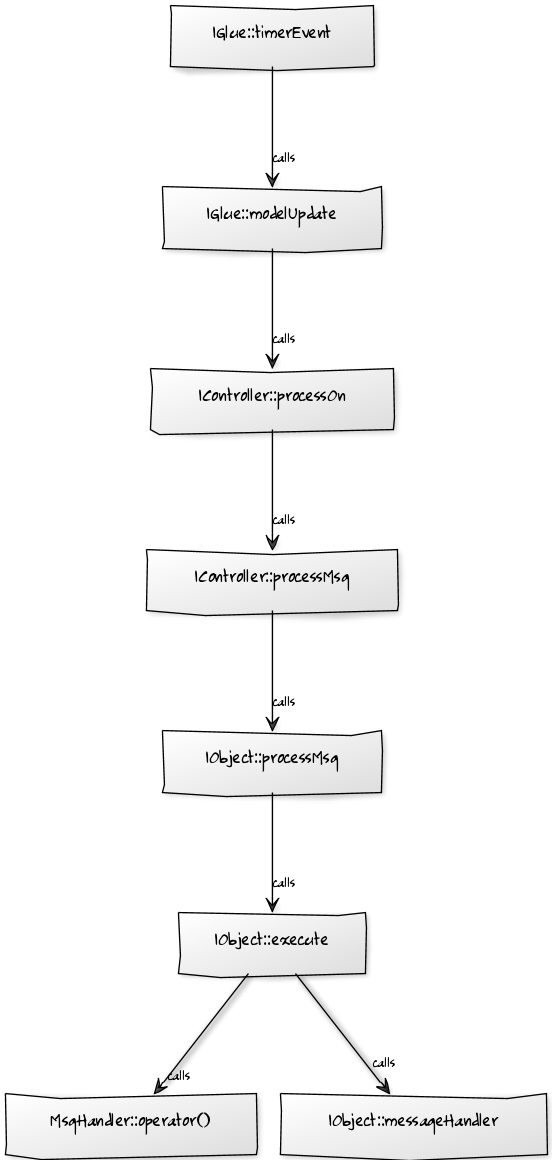
\includegraphics[height=18cm]{img/schema1.png}
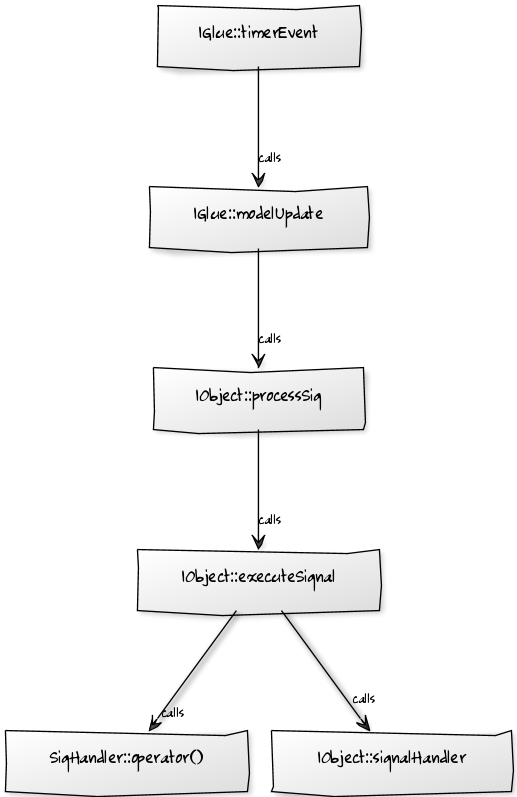
\includegraphics[height=18cm]{img/schema2.png}
\caption{Mechanisms for messages handlers and signals handlers}
\label{fig:handler}
\end{figure}

The methods available to connections with signals will be stored in a new fSignalHandlerMap in the IObject class, similar to the fMsgHandlerMap or the fGetMsgHandlerMap. This map will be similar to the existing ones, but will only be concerning the setting methods of attributes that can be connected to signals :

\begin{itemize}
  \item width, height
  \item (d)scale
  \item (d)x, (d)y, (d)z, (d)xorigin, (d)yorigin
  \item (d)angle
  \item rotatex, rotatey
  \item (d)red, (d)green, (d)blue, (d)hue, (d)saturation, (d)brightness, (d)alpha
  \item (d)date, (d)duration
  \item pen(d)Alpha, penWidth
\end{itemize}

Some attributes will not be taken into account at first, but could be in the future, such as \OSC{clock}, or \OSC{show}. The \OSC{clock} message does not take any value, and the \OSC{show} message expects a boolean.

In both cases, we could imagine a trigger that would send a \OSC{clock} message, or that would set the \OSC{show} message as \OSC{true} or \OSC{false}. The trigger value(s) could be set using the range parameters : when the signal values get out of these bounds, the message is triggered.

% grid : columns/rows
% guido : page, columns/rows


\bibliographystyle{unsrt}
%\bibliography{interlude}

\end{document}